\documentclass[conference]{IEEEtran}
\usepackage{cite}
\usepackage{amsmath,amssymb,amsfonts}
\usepackage{algorithmic}
\usepackage{graphicx}
\usepackage{textcomp}
\usepackage{xcolor}
\usepackage[hyphens]{url}
\usepackage[braket, qm]{qcircuit}
\usepackage{cleveref}
\usepackage{subcaption}
\usepackage{algorithm}

\crefname{section}{§}{§§}
\crefname{figure}{Fig.}{Fig.}
\crefname{algorithm}{Alg.}{Alg.}
\crefname{table}{Table}{Table}

\def\BibTeX{{\rm B\kern-.05em{\sc i\kern-.025em b}\kern-.08em
    T\kern-.1667em\lower.7ex\hbox{E}\kern-.125emX}}

% Ensure letter paper
\pdfpagewidth=8.5in
\pdfpageheight=11in

%%%%%%%%%%%---SETME-----%%%%%%%%%%%%%
\newcommand{\iscasubmissionnumber}{1}
%%%%%%%%%%%%%%%%%%%%%%%%%%%%%%%%%%%%

\pagenumbering{arabic}

%%%%%%%%%%%---SETME-----%%%%%%%%%%%%%
\title{An Implementation of the Quantum Verification of Matrix Products Algorithm}
\author{\normalsize{ISCA 2022 Submission
    \textbf{\#\iscasubmissionnumber} -- Confidential Draft -- Do NOT Distribute!!}}
%%%%%%%%%%%%%%%%%%%%%%%%%%%%%%%%%%%%

\begin{document}
\maketitle
\thispagestyle{plain}
\pagestyle{plain}


% TODO iterate on abstract

%%%%%% -- PAPER CONTENT STARTS-- %%%%%%%%

\begin{abstract}

  We present a space-efficient implementation of the quantum verification of
  matrix products (QVMP) algorithm and demonstrate its functionality by running
  it on the Aer simulator with two simulation methods: statevector and matrix
  product state (MPS). We report circuit metrics (gate count, qubit count,
  circuit depth), transpilation time, simulation time, and a proof of Grover
  oracle correctness.  Our study concludes that while QVMP can be simulated on
  moderately sized inputs, it cannot scale to a degree where we can observe any
  quantum advantage on current quantum hardware due to circuit depth and qubit
  count constraints. Further, the choice of simulation method has a noticeable
  impact on the size of the transpiled circuit which slows down development.

\end{abstract}

\section{Introduction}

  Grover's algorithm depends on a user-provided oracle that acts as a decision
  function over the input space. The oracle typically does not depend on quantum
  effects and can be programmed using classical operators. However, to use such
  an oracle in Grover's algorithm, we need to encode it as a quantum circuit.
  Programming reversible oracles can be tricky. It is difficult to reason about
  entanglement, non-trivial to debug, and cumbersome to formally verify
  correctness using machine-checked proofs.

  REVS \cite{amy2017verified} and Quipper \cite{green2013quipper} have presented
  compilers that can convert oracles written in a high-level classical language
  to reversible circuits using variants of Bennett's method.  To our knowledge,
  however, their work does not adequately address the space of compiling
  higher-level data structures like records, lists, and multi-dimensional
  arrays. There are interesting design choices to be made which can have an
  impact on the size and efficiency of the resulting circuit.

  In this study we demonstrate one such design choice by presenting an
  implementation of the Grover search based version of QVMP
  \cite{ambainis2002quantummatrix}. This algorithm runs in $O(n^{\frac{7}{4}})$
  time and improves upon the optimal classical bound provided by Freivalds
  \cite{freivalds1979fast}. Our implementation makes use of Quantum Read-Only
  Memory (QROM) \cite{babbush2018encoding} to efficiently encode the inputs,
  resulting in a quadratic improvement in space-efficiency ($O(n + m)$ qubits).
  
\section{Implementation}

The algorithm we implemented is summarized in \cref{alg:qvmp_grover}.
\cref{fig:qvmp_oracle_4x4} shows an example circuit that performs one iteration
of the Grover operator used in step 2.3. The sub-circuits used are QROM (denoted
by $db$), out-of-place inner product (denoted by $dot$), and diffuser.

\begin{algorithm}
  \caption{Quantum VMP using Grover Search ~\cite{lanl2018quantum}}
  \label{alg:qvmp_grover}
  \textbf{Input: } $n \times n$ matrices $A, B, C$ \\
  \textbf{Output: } 1 if $AB = C$ and 0 otherwise \\
  \textbf{Procedure: }
  \begin{enumerate}
    \item Partition $B$ and $C$ into sub-matrices of size $n \times \sqrt{n}$
    \item 
      {
        Perform amplitude amplification for $n^{\frac{1}{4}}$ iterations using this subroutine:
        \begin{enumerate}
          \item Pick a random vector $x$ of size $\sqrt{n}$
          \item Classically compute $y = B_ix$ and $z = C_ix$
          \item Using Grover search with $\sqrt{n}$ iterations, find a row of
            index $j$ such that $(Ay \neq z)_j$
        \end{enumerate}
      }
    \item XOR the sub-results
  \end{enumerate}
\end{algorithm}


\section{Results}

\begin{table*}
    \centering
    \begin{subtable}{\textwidth}
      \resizebox{\textwidth}{!}{%
        \begin{tabular}{|l|c||c|c|c|c|c|c|c|c||c|c|c|c|}
          \hline
          Dimension & Mismatches & ccx &      cx &   x &     h & z &      u1 &    u2 & u3 & Grover iterations &   Depth & Qubits & Total gates \\
          \hline
           (4, 4) &          1 &  30 &       1 &  11 &     2 & 1 &       2 &     2 &  0 &                 1 &      44 &     11 &          49 \\
          (16, 8) &          2 &  32 &   10108 &  69 &   284 & 2 &    8460 &  2536 &  3 &                 2 &   16993 &     21 &       21494 \\
          (32, 8) &          1 &  64 &   91408 & 272 &   997 & 4 &   91377 &  1056 &  8 &                 4 &  150375 &     22 &      185186 \\
         (32, 32) &          3 & 128 &  185912 & 151 &  2025 & 2 &  185897 &  2052 &  4 &                 2 &  303901 &     70 &      376171 \\
         (64, 16) &          2 & 128 &  786960 & 538 &  4190 & 4 &  786948 &  4232 &  5 &                 4 & 1300351 &     39 &     1583005 \\
         (64, 64) &          3 & 384 & 2329596 & 432 & 12396 & 3 & 2329587 & 12426 &  4 &                 3 & 3843672 &    135 &     4684828 \\
          \hline
        \end{tabular}}
      \caption{MPS}
      \label{table:circuit_metrics_mps}
    \end{subtable}
    \begin{subtable}{\textwidth}
      \resizebox{\textwidth}{!}{%
        \begin{tabular}{|l|c||c|c|c|c|c|c|c|c||c|c|c|c|}
          \hline
          Dimension & Mismatches & ccx &      cx &   x &     h & z &      u1 &    u2 & u3 & Grover iterations &   Depth & Qubits & Total gates \\
          \hline
          (4, 4) &          1 &  30 &  1 &  11 & 2 & 1 &  2 &  2 &  0 &                 1 &    44 &     11 &          49 \\
         (16, 4) &          2 &  16 &  0 &  75 & 4 & 2 &  3 & 12 &  1 &                 2 &   261 &     13 &         113 \\
         (16, 8) &          2 &  32 &  0 &  76 & 4 & 2 &  3 & 12 &  1 &                 2 &   385 &     21 &         130 \\
         (32, 4) &          2 &  24 &  0 & 208 & 5 & 3 &  4 & 24 &  2 &                 3 &   684 &     14 &         270 \\
         (64, 8) &          3 &  48 &  0 & 405 & 6 & 3 &  4 & 30 &  2 &                 3 &  2040 &     23 &         498 \\
         (64, 8) &          1 &  96 &  0 & 801 & 6 & 6 &  7 & 60 &  5 &                 6 &  4077 &     23 &         981 \\
          \hline
        \end{tabular}}
      \caption{Statevector}
      \label{table:circuit_metrics_statevector_cpu}
    \end{subtable}
    \caption{Circuit metrics for MPS and statevector simulation methods on
    select dimensions. Depth and total gates were measured after transpilation.}
    \label{table:circuit_metrics}
  \end{table*}


\subsection{Functionality}

\begin{figure}
  \centering
  \begin{subfigure}{0.48\textwidth}
    \centering
    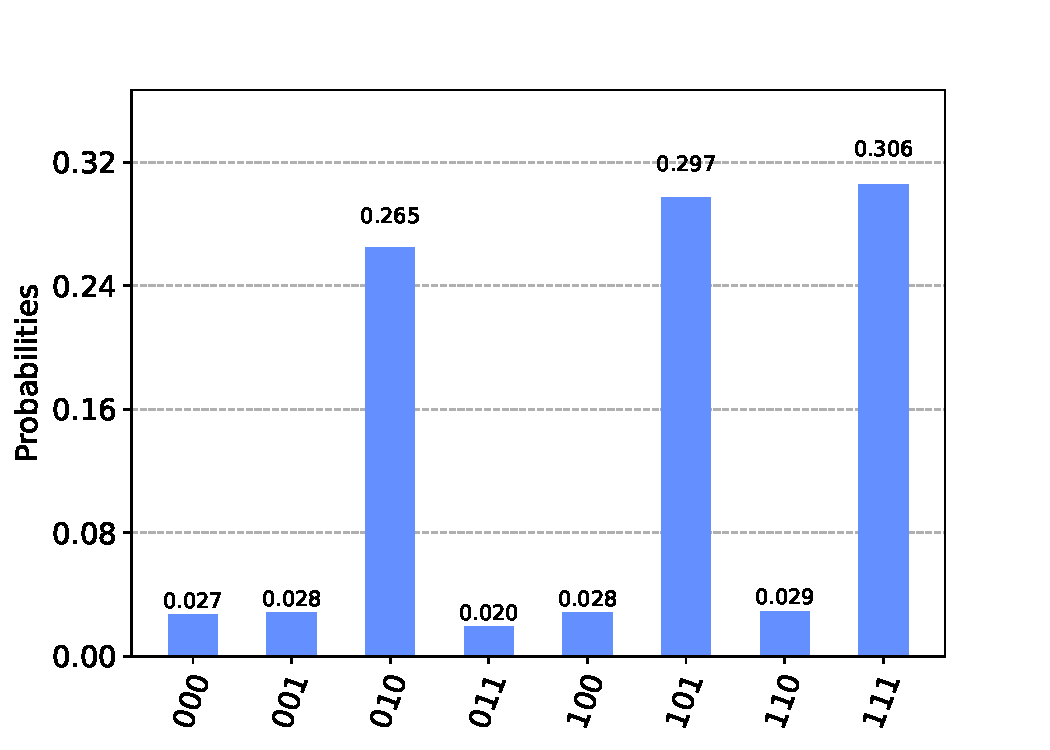
\includegraphics[width=0.6\textwidth]{../../results/figures/qvmp_functionality_found_unknown.pdf}
    \caption{\textbf{Success}: $8 \times 8$ matrix with $(Ay \neq z)_j$ for $j \in \{2, 5, 7\}$}
    \label{fig:qvmp_functionality_success}
  \end{subfigure}
  \begin{subfigure}{0.48\textwidth}
    \centering
    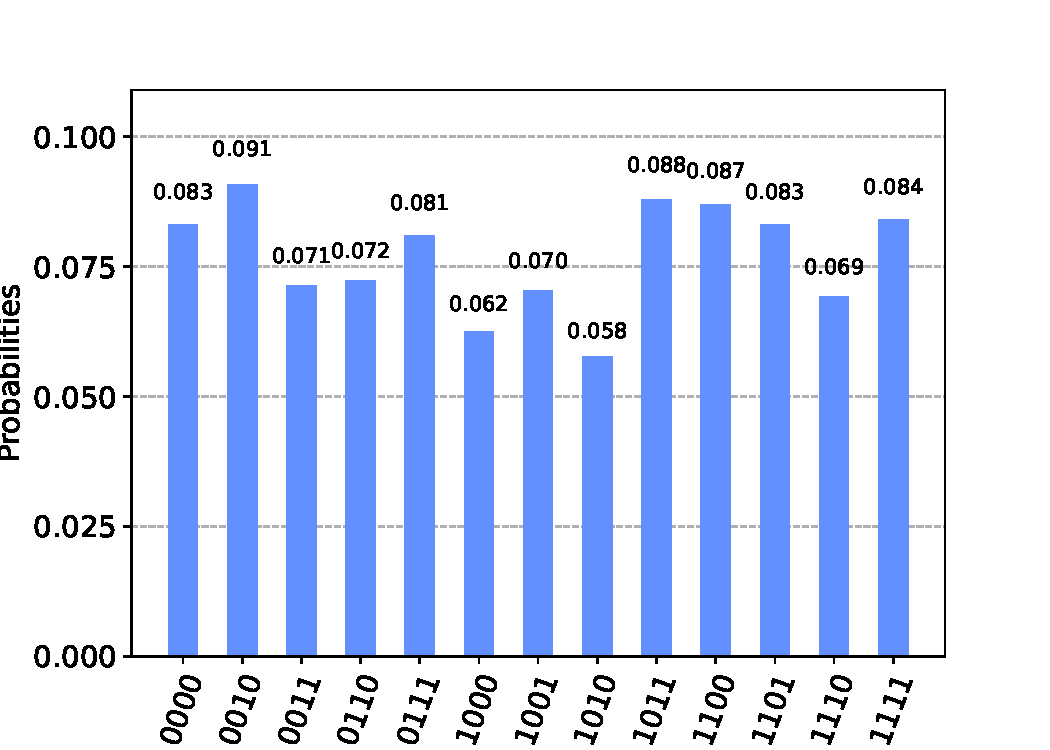
\includegraphics[width=0.6\textwidth]{../../results/figures/qvmp_functionality_pfound_unknown__1.pdf}
    \caption{\textbf{Failure}: $16 \times 16$ matrix with $(Ay \neq z)_j$ for $j \in \{1, 4, 5\}$}
    \label{fig:qvmp_functionality_failure}
  \end{subfigure}
  \caption{Histogram showing the probability distribution of measuring the
  address qubits of the QVMP circuit}
  \label{fig:qvmp_functionality}
\end{figure}

\cref{fig:qvmp_functionality_success} demonstrates that our implementation is
able to correctly find the row indices where there is a mismatch.
\cref{fig:qvmp_functionality_failure} demonstrates a failure case that happens
when the number of Grover iterations prescribed by the algorithm is not a
multiple of period, which we define to be the number of oscillations between the
Grover-optimal number of iterations.

\subsection{Circuit Metrics}

We report circuit metrics (gate count, circuit depth, qubit count)
\cref{table:circuit_metrics} measured when using the MPS and statevector methods
for the Grover search portion of QVMP (step 2.3 in \cref{alg:qvmp_grover}. The
metrics are reported on circuits that used the optimal number of Grover
iterations. When using the statevector method we see a small decrease in the
circuit depth. Using MPS, on the other hand, results in two to three orders of
magnitude more gate count and circuit depth.

\subsection{Transpilation and Simulation}

\begin{figure}[h!]
  \begin{subfigure}{0.48\textwidth}
    \centering
    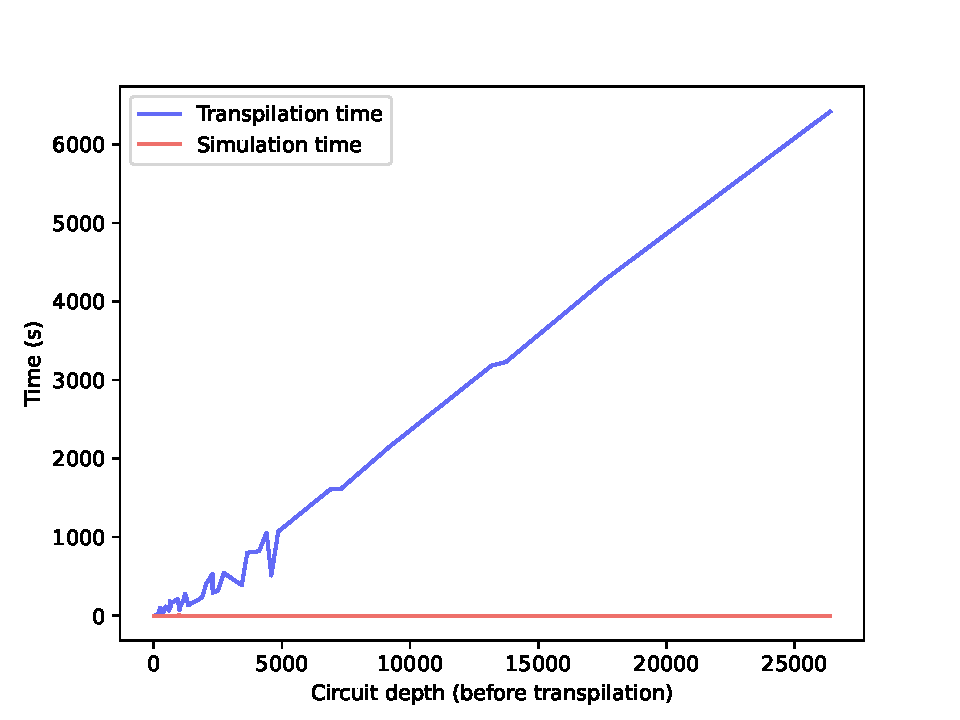
\includegraphics[width=0.6\textwidth]{../../results/figures/circuit_depth_v_tran_time_and_sim_time-MPS.pdf}
    \caption{MPS}
  \end{subfigure}
  \begin{subfigure}{0.48\textwidth}
    \centering
    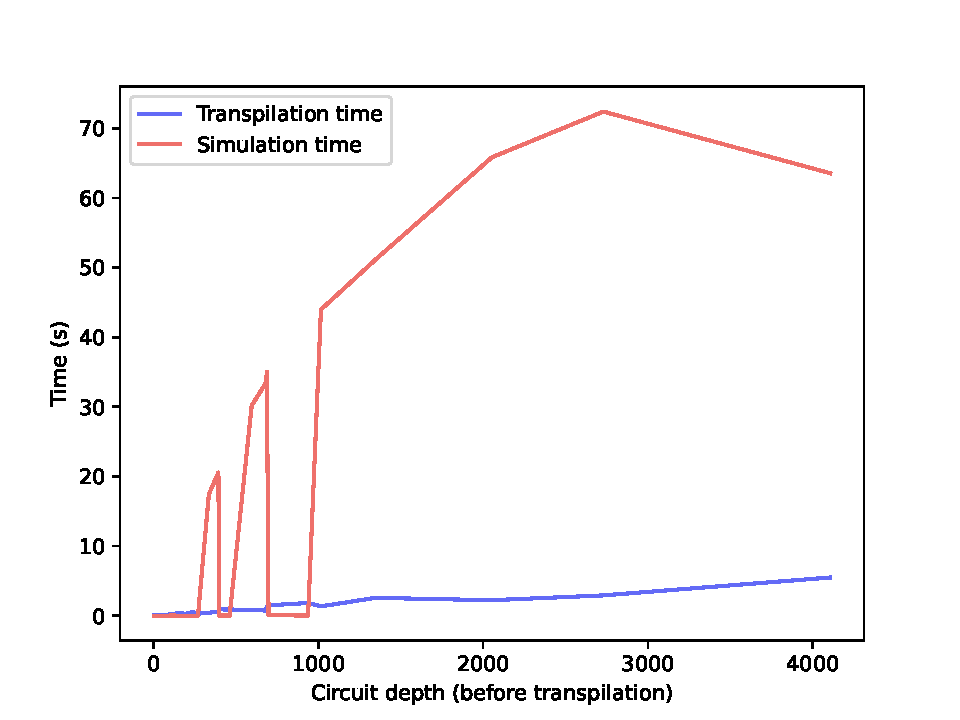
\includegraphics[width=0.6\textwidth]{../../results/figures/circuit_depth_v_tran_time_and_sim_time-statevector_cpu.pdf}
    \caption{Statevector}
  \end{subfigure}
  \caption{Circuit depth vs Transpilation/Simulation time}
  \label{fig:circuit_depth_of_trans_v_sim}
\end{figure}

\cref{fig:circuit_depth_of_trans_v_sim} showcases how transpilation time and
simulation time change as the circuit depth increases.  MPS seems to be spending
more time on transpilation while its simulation time remains mostly constant.
Statevector spends more time during simulation with transpilation time growing
at a slow rate.

\begin{figure*}
  \centering
  \scalebox{1}{\scalebox{1.0}{
\Qcircuit @C=1.0em @R=0.2em @!R { \\
	 	\nghost{{address}_{0} :  } & \lstick{{address}_{0} :  } & \gate{\mathrm{H}} \barrier[0em]{10} & \qw & \multigate{10}{\mathrm{db}}_<<<{0} & \qw & \qw & \qw & \multigate{10}{\mathrm{db\_dg}}_<<<{0} \barrier[0em]{10} & \qw & \multigate{1}{\mathrm{diffuser}}_<<<{0} \barrier[0em]{10} & \qw & \meter & \qw & \qw & \qw\\
	 	\nghost{{address}_{1} :  } & \lstick{{address}_{1} :  } & \gate{\mathrm{H}} & \qw & \ghost{\mathrm{db}}_<<<{1} & \qw & \qw & \qw & \ghost{\mathrm{db\_dg}}_<<<{1} & \qw & \ghost{\mathrm{diffuser}}_<<<{1} & \qw & \qw & \meter & \qw & \qw\\
	 	\nghost{{a}_{0} :  } & \lstick{{a}_{0} :  } & \qw & \qw & \ghost{\mathrm{db}}_<<<{2} & \multigate{8}{\mathrm{dot}}_<<<{0} & \qw & \multigate{8}{\mathrm{dot\_dg}}_<<<{0} & \ghost{\mathrm{db\_dg}}_<<<{2} & \qw & \qw & \qw & \qw & \qw & \qw & \qw\\
	 	\nghost{{a}_{1} :  } & \lstick{{a}_{1} :  } & \qw & \qw & \ghost{\mathrm{db}}_<<<{3} & \ghost{\mathrm{dot}}_<<<{1} & \qw & \ghost{\mathrm{dot\_dg}}_<<<{1} & \ghost{\mathrm{db\_dg}}_<<<{3} & \qw & \qw & \qw & \qw & \qw & \qw & \qw\\
	 	\nghost{{a}_{2} :  } & \lstick{{a}_{2} :  } & \qw & \qw & \ghost{\mathrm{db}}_<<<{4} & \ghost{\mathrm{dot}}_<<<{2} & \qw & \ghost{\mathrm{dot\_dg}}_<<<{2} & \ghost{\mathrm{db\_dg}}_<<<{4} & \qw & \qw & \qw & \qw & \qw & \qw & \qw\\
	 	\nghost{{a}_{3} :  } & \lstick{{a}_{3} :  } & \qw & \qw & \ghost{\mathrm{db}}_<<<{5} & \ghost{\mathrm{dot}}_<<<{3} & \qw & \ghost{\mathrm{dot\_dg}}_<<<{3} & \ghost{\mathrm{db\_dg}}_<<<{5} & \qw & \qw & \qw & \qw & \qw & \qw & \qw\\
	 	\nghost{{y}_{0} :  } & \lstick{{y}_{0} :  } & \gate{\mathrm{X}} & \qw & \ghost{\mathrm{db}} & \ghost{\mathrm{dot}}_<<<{4} & \qw & \ghost{\mathrm{dot\_dg}}_<<<{4} & \ghost{\mathrm{db\_dg}} & \qw & \qw & \qw & \qw & \qw & \qw & \qw\\
	 	\nghost{{y}_{1} :  } & \lstick{{y}_{1} :  } & \gate{\mathrm{X}} & \qw & \ghost{\mathrm{db}} & \ghost{\mathrm{dot}}_<<<{5} & \qw & \ghost{\mathrm{dot\_dg}}_<<<{5} & \ghost{\mathrm{db\_dg}} & \qw & \qw & \qw & \qw & \qw & \qw & \qw\\
	 	\nghost{{y}_{2} :  } & \lstick{{y}_{2} :  } & \qw & \qw & \ghost{\mathrm{db}} & \ghost{\mathrm{dot}}_<<<{6} & \qw & \ghost{\mathrm{dot\_dg}}_<<<{6} & \ghost{\mathrm{db\_dg}} & \qw & \qw & \qw & \qw & \qw & \qw & \qw\\
	 	\nghost{{y}_{3} :  } & \lstick{{y}_{3} :  } & \qw & \qw & \ghost{\mathrm{db}} & \ghost{\mathrm{dot}}_<<<{7} & \qw & \ghost{\mathrm{dot\_dg}}_<<<{7} & \ghost{\mathrm{db\_dg}} & \qw & \qw & \qw & \qw & \qw & \qw & \qw\\
	 	\nghost{{z} :  } & \lstick{{z} :  } & \qw & \qw & \ghost{\mathrm{db}}_<<<{6} & \ghost{\mathrm{dot}}_<<<{8} & \gate{\mathrm{Z}} & \ghost{\mathrm{dot\_dg}}_<<<{8} & \ghost{\mathrm{db\_dg}}_<<<{6} & \qw & \qw & \qw & \qw & \qw & \qw & \qw\\
	 	\nghost{\mathrm{{data} :  }} & \lstick{\mathrm{{data} :  }} & \lstick{/_{_{2}}} \cw & \cw & \cw & \cw & \cw & \cw & \cw & \cw & \cw & \cw & \dstick{_{_{\hspace{0.0em}0}}} \cw \ar @{<=} [-11,0] & \dstick{_{_{\hspace{0.0em}1}}} \cw \ar @{<=} [-10,0] & \cw & \cw\\
\\ }}
}
  \caption{QVMP circuit for a $4 \times 4$ matrix $A$ performing one iteration}
  \label{fig:qvmp_oracle_4x4}
\end{figure*}

\section{Conclusions}

In this study we present an implementation of QVMP in Qiskit that uses $O(n+m)$
qubits achieved by using QROM to encode inputs. We reported circuit metrics
(gate count, depth, qubit count) as well as transpilation and simulation times.
While QVMP can be simulated (and even run) on moderately-sized inputs, it
cannot, with present hardware, scale to a degree where we can observe any
quantum advantage. We demonstrate that the choice of simulation method has a
noticeable impact on depth of the circuit, the effects of which trickle into
transpilation and simulation time.

\section*{Acknowledgements}

This research was supported in part through research infrastructure and services
provided by the Rogues Gallery testbed \cite{young:2019:rg-exp-insights} hosted
by the Center for Research into Novel Computing Hierarchies (CRNCH) at Georgia
Tech.


%%%%%%% -- PAPER CONTENT ENDS -- %%%%%%%%


%%%%%%%%% -- BIB STYLE AND FILE -- %%%%%%%%
\bibliographystyle{IEEEtranS}
\bibliography{refs}
%%%%%%%%%%%%%%%%%%%%%%%%%%%%%%%%%%%%



\end{document}

